\documentclass[11pt]{article}
\usepackage{latexsym}
\usepackage{amsmath}
\usepackage{amssymb}
\usepackage{amsthm}
\usepackage{epsfig}
\usepackage[tight]{subfigure}

% TD (Nitish)
%   online policy evaluation
%   learning rate, intuition and bounds (Mike)
% SARSA (Nitish)
%   define the loss function
%   derive the full gradient 
%   drop the extra term
%   explain that this is NOT gradient descent
%   mention the Bellman-Residual method
% Q-Learning (Mike)
%   online fitted Q-iteration
%   restate the parameter update
%   exploration policies: epsilon-greedy and Boltzman
% Off-Policy vs On-Policy learning (Mike)
% Experience Replay (Mike)


%extra packages added
%\usepackage{algorithm}
%\usepackage{algorithmic}
\numberwithin{equation}{section}
\numberwithin{figure}{section}

\newcommand{\handout}[5]{
  \noindent
  \begin{center}
  \framebox{
    \vbox{
      \hbox to 5.78in { {#1} \hfill #2 }
      \vspace{4mm}
      \hbox to 5.78in { {\Large \hfill #5  \hfill} }
      \vspace{2mm}
      \hbox to 5.78in { {\em #3 \hfill #4} }
    }
  }
  \end{center}
  \vspace*{4mm}
}

\newcommand{\lecture}[5]{\handout{#1}{#2}{#3}{#4}{#5}}

\newtheorem{theorem}{Theorem}
\newtheorem{corollary}[theorem]{Corollary}
\newtheorem{lemma}[theorem]{Lemma}
\newtheorem{observation}[theorem]{Observation}
\newtheorem{proposition}[theorem]{Proposition}
\newtheorem{definition}[theorem]{Definition}
\newtheorem{claim}[theorem]{Claim}
\newtheorem{fact}[theorem]{Fact}
\newtheorem{assumption}[theorem]{Assumption}

% 1-inch margins, from fullpage.sty by H.Partl, Version 2, Dec. 15, 1988.
\topmargin 0pt
\advance \topmargin by -\headheight
\advance \topmargin by -\headsep
\textheight 8.9in
\oddsidemargin 0pt
\evensidemargin \oddsidemargin
\marginparwidth 0.5in
\textwidth 6.5in

\parindent 0in
\parskip 1.5ex

%\renewcommand{\baselinestretch}{1.25}

\begin{document}

%%%%%%%%%%%%%%%%%%%%%%%%%%%%%%%%%%%%%%%%%%%%%%%%%%%%
% Document header: change the lecture number, date, scribe name, and
% lecture topic.
%%%%%%%%%%%%%%%%%%%%%%%%%%%%%%%%%%%%%%%%%%%%%%%%%%%%
%\lecture{Statistical Techniques in Robotics (16-831, F10)}
%{Lecture\#NN (Thursday August 26)}
%{Lecturer: Drew Bagnell}
%{Scribe:YOUR\_NAME\_HERE \footnotemark}
%{Lecture Topic}

\lecture{Statistical Techniques in Robotics (16-899, S14)}%
{Lecture \#09, (Feb. 11, 2014)}%
{Lecturer: Drew Bagnell}%
{Scribes: Michael Koval and Nitish Thatte}%
{Q-Learning}

% Be sure to acknowledge all previous scribes.
\footnotetext[1]{Some content adapted from previous scribe: Jackie Libby}

%%%%%%%%%%%%%%%%%%%%%%%%%%%%%%%%%%%%%%%%%%%%%%%%%%%%
% Document body: Scribe your notes here.
%%%%%%%%%%%%%%%%%%%%%%%%%%%%%%%%%%%%%%%%%%%%%%%%%%%%

%%%%%%%%%%%%%%%%%%%%%%%%%%%%%%%%%%%%%%%%%%%%%%%%%%%%
\section{Overview}
%%%%%%%%%%%%%%%%%%%%%%%%%%%%%%%%%%%%%%%%%%%%%%%%%%%%
In the last few lectures we covered several offline batch methods such as Fitted Value Iteration, Fitted Q-Iteration, and Approximate Policy Iteration.  While these methods make efficient use of available training data, they may suffer due to their potentially high memory consumption. In this lecture, we present online techniques that can perform well even when presented with large amounts of data, as in the case of samples generated by simulations. With these online techniques, we perform an update after sampling each data tuple.  The following block diagram generalizes this idea.

\begin{figure}[h!]
	\centering
	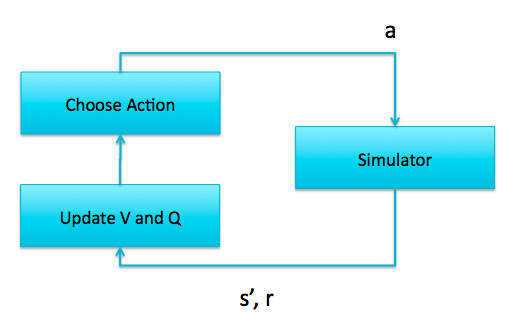
\includegraphics[width=.4\columnwidth]{./images/figBlock}
	%\caption{}
	\label{fig.figBlock}
\end{figure}

First we will present the Temporal Differencing method for online updates in the context of policy evaluation. Then, we will look at approximate methods such as SARSA and Q-learning.
%%%%%%%%%%%%%%%%%%%%%%%%%%%%%%%%%%%%%%%%%%%%%%%%%%%%

\section{Temporal Differencing (TD)}
%%%%%%%%%%%%%%%%%%%%%%%%%%%%%%%%%%%%%%%%%%%%%%%%%%%%
% TODO: Explain that Eqn. 2.1 is policy evaluation, not TD.
Equation~\ref{eq.policyEval} is 
\begin{equation}
	V_\pi(s) = R(s,\pi(s)) + \gamma E_{s'}[V_\pi(s')]
	\label{eq.policyEval}
\end{equation}

%%%%%%%%%%%%%%%%%%%%%%%%%%%%%%%%%%%%%%%%%%%%%%%%%%%%
\subsection*{Algorithm TD:}

\begin{enumerate}
	\item Initialize $V$
	\item $\forall s$, repeat until $V$ converges
	\begin{enumerate}
		\item Initialize $s$
		\item Repeat until $s$ is terminal (This is a trajectory from a particular intitial starting state.)
		\begin{enumerate}
			\item Do $\pi(s)$
			\item Observe $s', r$
			\item Update ($V, s, r, s'$)
			\label{step.updateTD}
			\item $s \leftarrow s'$
		\end{enumerate}		
	\end{enumerate}		
\end{enumerate}		

Let's look at the Udpate rule in step \ref{step.updateTD} a little more closely.  We can look at both the tabular cases, and when we have a function approximator.

%%%%%%%%%%%%%%%%%%%%%%%%%%%%%%%%%%%%%%%%%%%%%%%%%%%%
\subsection*{TD Update for Tabular Case}
% TODO: Start with 2.3
% TODO: Also add the {i} and {i + 1} indices.
% TODO: Derive the full gradient; drop the necessary term.
% TODO: Discuss annealing of alpha and the convergence properties.
% TODO: Explain what \alpha is.
% TODO: Replace V with \tilde{V}^\pi.
Given $V, s, r, s'$, update $V(s)$ (the value in our table).  We use $\alpha$ as a proportiality factor, and we approximate the new value as a proportion of the old value summed with a proportion of the value as estimated from Eq. (\ref{eq.valueTD}).  From Eq. (\ref{eq.valueTD}), we approximate $E_{s'}[V_\pi(s')]$ with $V(s')$.  And so we get:
\begin{equation}
	V_\pi(s) \leftarrow (1-\alpha)V(s) + \alpha(r+\gamma V(s')), \alpha \in [0,1]
	\label{eq.updateTD}
\end{equation}
We can define the loss as:
\begin{equation}
	L = \frac{1}{2}(V_\pi(s)-V(s))^2
\end{equation}
We want our update rule to move in the negative direction of the gradient of the loss:
\begin{equation}
	V(s) \leftarrow V(s) - \alpha \frac{\partial L}{\partial V(s)}
\end{equation}
The gradient is:
\begin{equation}
	\frac{\partial L}{\partial V(s)} = -(V_\pi(s) - V(s))
	\label{eq.gradientLoss}
\end{equation}
We can get the value of this gradient by rearranging terms from Eq. (\ref{eq.updateTD}):
\begin{equation}
	-(V_\pi(s) - V(s)) = -(r + \gamma V(s') - V(s))
\end{equation}
And so finally our update rule is:
\begin{equation}
	V_\pi(s) \leftarrow V(s) + \alpha (r + \gamma V(s') - V(s))
	\label{eq.updateTDFinal}
\end{equation}
For shorthand, let 
\begin{equation}
	\delta = (r + \gamma V(s') - V(s)),
	\label{eq.delta}
\end{equation}
so we can re-write the update as:
\begin{equation}
	V_\pi(s) \leftarrow V(s) + \alpha \delta
	\label{eq.updateTDShort}
\end{equation}
%%%%%%%%%%%%%%%%%%%%%%%%%%%%%%%%%%%%%%%%%%%%%%%%%%%%
\subsection*{TD Update with Function Approximator}
Now let's look at the parametric case.  Let $\theta$ be the parameter, so we have $V_\theta(s)$.  For example, if we have a linear function, in might be:
\begin{equation}
	V_\theta(s) = \theta^TF(s)
\end{equation}
For the gradient of the loss, we must now use the chain rule, replacing Eq. (\ref{eq.gradientLoss}) with:
\begin{equation}
	\frac{\partial L}{\partial V(s)} = -(V_\pi(s) - V(s))\bigtriangledown_\theta V_\theta(s)
\end{equation}
Then our update becomes,
\begin{equation}
	\theta \leftarrow \theta + \alpha \delta \bigtriangledown_\theta V_\theta(s),
\end{equation}
with $\delta$ as defined in Eq. (\ref{eq.delta}).

%%%%%%%%%%%%%%%%%%%%%%%%%%%%%%%%%%%%%%%%%%%%%%%%%%%%
\subsection*{Grid-based world example:}
The diagram below shows a grid-based world, where the robot starts in the upper left, and the goal is in the lower right.  The robot gets a reward of $+1$ if it reaches the goal, and $0$ everywhere else.  There is a discount factor of $\gamma$.  The policy is for the robot to go right until it reaches the wall, and then go down.
\begin{figure}[h!]
	\centering
	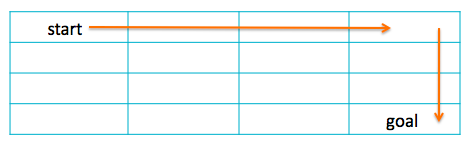
\includegraphics[width=.4\columnwidth]{./images/fig1}
	%\caption{}
	\label{fig.fig1}
\end{figure}

We start by initializing all states to 0:

\begin{figure}[h!]
	\centering
	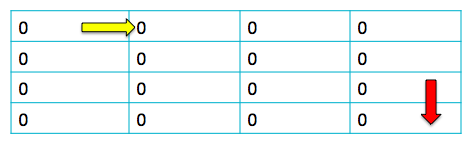
\includegraphics[width=.4\columnwidth]{./images/fig2}
	%\caption{}
	\label{fig.fig2}
\end{figure}

As the robot moves one cell over from the start state (yellow arrow above), the reward is $0$, and the value of both the current state and the next state is $0$, so $\delta$ evaluates to $0$.  (See Eq. \ref{eq.delta}).  As the robot moves into the goal state (red arrow), the reward is $1$, so $\delta$ evaluates to $1$.  We then update the second-to-last cell with Eq. (\ref{eq.updateTDShort}) and we get:

\begin{figure}[h!]
	\centering
	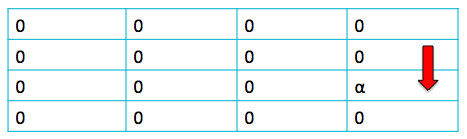
\includegraphics[width=.4\columnwidth]{./images/fig3}
	%\caption{}
	\label{fig.fig3}
\end{figure}

Another iteration of the algorithm gives us:

\begin{figure}[h!]
	\centering
	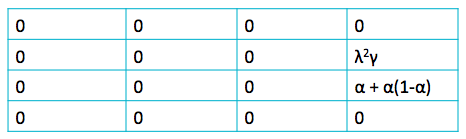
\includegraphics[width=.4\columnwidth]{./images/fig4}
	%\caption{}
	\label{fig.fig4}
\end{figure}

This method is slow, because we have to run the whole policy just to update the next cell.  Instead, when we update a cell, we could iterate all the way backwards, tracing back to the start location, updating values as we go.  This is the idea behind eligibility traces, as disucssed below.

%%%%%%%%%%%%%%%%%%%%%%%%%%%%%%%%%%%%%%%%%%%%%%%%%%%%
\section{Eligibility Traces}
%%%%%%%%%%%%%%%%%%%%%%%%%%%%%%%%%%%%%%%%%%%%%%%%%%%%
Let $e(s)$ be out elibility trace, which is a proportional elibility factor.
Then our update becomes:
\begin{equation}
	V(s") \leftarrow + \alpha \delta e(s"), \forall s"
\end{equation}

%%%%%%%%%%%%%%%%%%%%%%%%%%%%%%%%%%%%%%%%%%%%%%%%%%%%
\subsection*{Algorithm TD($\lambda$):}
\begin{enumerate}
	\item Initialize $V$
	\item $\forall s$, repeat until $V$ converges
	\begin{enumerate}
		\item Initialize $s$
		\item $\forall s', e(s') = 0$
		\item Repeat until $s$ is terminal
		\begin{enumerate}
			\item Do $\pi(s)$
			\item Observe $s', r$
			\item $e(s) \leftarrow e(s) + 1$
			\label{step.elig}
			\item $\delta \leftarrow (r+\gamma V(s') - V(s))$
			\item $\forall$ states $s"$
			\label{step.forall}
			\begin{enumerate}
				\item $V(s") \leftarrow V(s") + \alpha \delta e(s")$
				\item $e(s") \leftarrow \lambda \gamma e(s")$
				\label{step.elig2}
			\end{enumerate}	
		\end{enumerate}		
	\end{enumerate}		
\end{enumerate}		
Note that if $\lambda = 0$, we just get the regular TD algorithm.

Using the same grid cell world example, we start by initializing the values and the eligibility of each state to $0$. (Values shown in black, eligibility shown in red.)

\begin{figure}[h!]
	\centering
	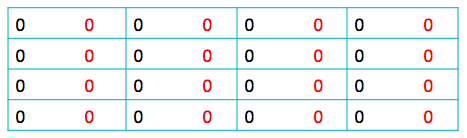
\includegraphics[width=.4\columnwidth]{./images/fig5}
	%\caption{}
	\label{fig.fig5}
\end{figure}

Updating the elgibility of the first cell with step \ref{step.elig}, we get:

\begin{figure}[h!]
	\centering
	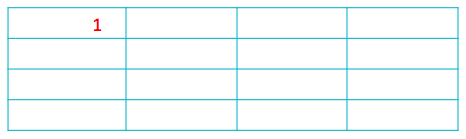
\includegraphics[width=.4\columnwidth]{./images/fig6}
	%\caption{}
	\label{fig.fig6}
\end{figure}

Below, the second cell has been updated with step \ref{step.elig}, and the first cell has been updated with step \ref{step.elig2}:
\clearpage
\begin{figure}[h]
	\centering
	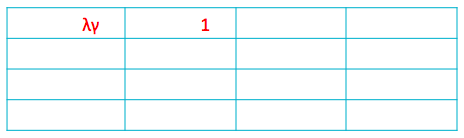
\includegraphics[width=.4\columnwidth]{./images/fig7}
	%\caption{}
	\label{fig.fig7}
\end{figure}

This is after updating both the first and second cell again with step \ref{step.elig2}:
\begin{figure}[h!]
	\centering
	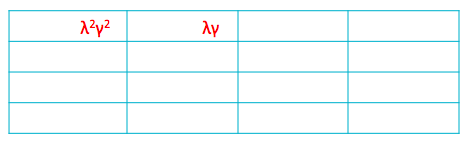
\includegraphics[width=.4\columnwidth]{./images/fig8}
	%\caption{}
	\label{fig.fig8}
\end{figure}

After completing all cells, we get:
\begin{figure}[h!]
	\centering
	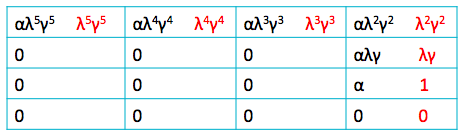
\includegraphics[width=.4\columnwidth]{./images/figFinal}
	%\caption{}
	\label{fig.figFinal}
\end{figure}

Note that as $\lambda \rightarrow 0$, the values will get smaller and smaller as we go further back to the start.

%%%%%%%%%%%%%%%%%%%%%%%%%%%%%%%%%%%%%%%%%%%%%%%%%%%%
\subsection*{TD($\lambda$) Update with Function Approximator}
In the parametric case, we change a couple steps in the TD($\lambda$) algorithm above.

Step \ref{step.elig} becomes
\begin{equation}
	e \leftarrow \lambda \gamma e + \bigtriangledown_\theta V_\theta(s)
\end{equation}

Step \ref{step.forall} becomes
\begin{equation}
	\theta \leftarrow \theta + \alpha \delta e,
\end{equation}
where
\begin{equation}
	e = \sum_{s"} e(s") \bigtriangledown_\theta V(s") 
\end{equation}
%%%%%%%%%%%%%%%%%%%%%%%%%%%%%%%%%%%%%%%%%%%%%%%%%%%%
\section{SARSA}
%%%%%%%%%%%%%%%%%%%%%%%%%%%%%%%%%%%%%%%%%%%%%%%%%%%%
In SARSA, we find our optimal policy $\pi^*$ by learning $Q^*$.  If we have an exact model, we can use the equation:
\begin{equation}
	Q^*(s,a) = R(s,a) + \gamma E_{p(s'|s,a)}[\max_{a'} Q^*(s',a')]
	\label{eq.sarsa}
\end{equation}
When we don't have an exact model, we estimate $Q^*$, which is what we'll do here.

With TD, we were operating on transitions between states.

With SARSA, we are operating on transitions between state, action pairs.
%%%%%%%%%%%%%%%%%%%%%%%%%%%%%%%%%%%%%%%%%%%%%%%%%%%%
\subsection*{Algorithm SARSA:}
\begin{enumerate}
	\item Initialize $Q$
	\item Repeat until $Q$ converges
	\begin{enumerate}
		\item Initialize $s$, $a \sim \hat{\pi}_{Q(s)}$

		(This means we initialize the action randomly according to some distribution $\hat{\pi}_{Q(s)}$.)
		\item Repeat until $s$ is terminal
		\begin{enumerate}
			\item Do $a$
			\item Observe $s'$, $r$
			\item Pick $a' \sim \hat{\pi}_{Q(s')}$
			\item Update ($Q, s, a, r, s', a'$)
			
			(This is where SARSA comes from!)
			\item $s \leftarrow s'$, $a \leftarrow a'$ 
		\end{enumerate}
	\end{enumerate}
\end{enumerate}

%%%%%%%%%%%%%%%%%%%%%%%%%%%%%%%%%%%%%%%%%%%%%%%%%%%%
\subsection*{defining $\hat{\pi}_Q$}
There are two ways that $\hat{\pi}_Q$ can be defined:
\begin{enumerate}
	\item $\varepsilon$ - greedy $\hat{\pi}_Q$
		\begin{equation}
			\hat{\pi}_Q(s) = 
			\begin{cases}
				\operatorname{arg\,max}_{a}Q(s,a) & \text{with probability } 1 - \varepsilon, \\
				\text{random action} & \text{with probability } \varepsilon.
			\end{cases}
		\end{equation}
	\item Boltzmann exploration
		\begin{equation}
			\hat{\pi}_Q(s,a) =\frac{\exp(\frac{Q(s,a)}{B})}{\sum_{a'}\exp(\frac{Q(s,a')}{B})}
		\end{equation}
		The denominator is a normalization factor.  If the $Q$ value of a certain action is high, then we pick that action with higher probability.  $B$ is a temperature term.  The higher the temperature, the closer to a uniform distribution, and so the less greedy.
\end{enumerate}

%%%%%%%%%%%%%%%%%%%%%%%%%%%%%%%%%%%%%%%%%%%%%%%%%%%%
\subsection*{SARSA Update for Tabular Case}
Eq. (\ref{eq.sarsa}) is the exact value of $Q$, if we have a model.  We approximate $Q$ with:
\begin{equation}
	Q(s,a) \leftarrow (1 - \alpha) Q(s,a) + \alpha(r + \gamma Q(s',a'))
	\label{eq.sarsaApprox}
\end{equation}
We can rewrite this as:
\begin{equation}
	Q(s,a) = Q(s,a) + \alpha(r + \gamma Q(s',a') - Q(s,a))
\end{equation}
let $\delta = (r + \gamma Q(s',a') - Q(s,a))$, so then we can write:
\begin{equation}
	Q(s,a) = Q(s,a) + \alpha \delta
	\label{eq.sarsaUpdateTab}
\end{equation}
%%%%%%%%%%%%%%%%%%%%%%%%%%%%%%%%%%%%%%%%%%%%%%%%%%%%
\subsection*{SARSA Update with Function Approximator}
For the parametric case, we change Eq. (\ref{eq.sarsaUpdateTab}) to:
\begin{equation}
	\theta \leftarrow \theta + \alpha \delta \bigtriangledown_\theta Q_\theta(s,a)
\end{equation}
For example, if $Q_\theta(s,a) = \theta^T f(s,a)$, then $\bigtriangledown_\theta Q_\theta(s,a) = f(s,a)$
%%%%%%%%%%%%%%%%%%%%%%%%%%%%%%%%%%%%%%%%%%%%%%%%%%%%
\subsection*{Algorithm SARSA($\lambda$):}
(SARSA with elibility trace)
\begin{enumerate}
	\item Initialize $Q$
	\item Repeat until $Q$ converges
	\begin{enumerate}
		\item Initialize $s$, $a \sim \hat{\pi}_\theta(s)$
		\item Repeat until $s$ is terminal
		\begin{enumerate}
			\item Do $a$
			\item Observe $s'$, $r$
			\item Pick $a' \sim \hat{\pi}_{Q(s')}$
			\item $e(s,a) \leftarrow e(s,a) + 1$
			\item $\delta \leftarrow (r + \gamma Q(s',a') - Q(s,a))$
			\item $\forall (s",a")$
			\begin{enumerate}
				\item $Q(s",a") \leftarrow Q(s",a") + \alpha \delta e(s",a")$
				\item $e(s",a") \leftarrow \lambda \gamma e(s",a")$	
			\end{enumerate}
		\end{enumerate}
	\end{enumerate}
\end{enumerate}

%%%%%%%%%%%%%%%%%%%%%%%%%%%%%%%%%%%%%%%%%%%%%%%%%%%%
\section{Q-learning}
%%%%%%%%%%%%%%%%%%%%%%%%%%%%%%%%%%%%%%%%%%%%%%%%%%%%
The only difference from SARSA is how we do the update.  Again, Eq. (\ref{eq.sarsa}) is the exact value of $Q$, if we have a model.  In SARSA, we approximated this with Eq. (\ref{eq.sarsaApprox}).  Now we approximate with:
\begin{equation}
	Q(s,a) \leftarrow (1 - \alpha) Q(s,a) + \alpha(r + \gamma \max_{a'}Q(s',a'))
\end{equation}
The only difference from Eq. (\ref{eq.sarsaApprox}) is the $\max$ term.  This allows us to pick actions without worrying about the policy distribution.
\end{document}
